\documentclass[conference]{IEEEtran}
\usepackage{graphicx}
\usepackage{booktabs}
\graphicspath{ {images/} }
\IEEEoverridecommandlockouts

    

\begin{document}


\title{Customer Segmentation Using K-Means and DBSCAN Clustering: A Comparative Study \\
{\footnotesize \textsuperscript{}}
\thanks{}
}
 

\author{\IEEEauthorblockN{ Abhishek Puppala}
\IEEEauthorblockA{\textit{Department of Information Science} \\
\textit{University of North Texas}\\
Texas, USA \\
AbhishekPuppala@my.unt.edu}
\and
\IEEEauthorblockN{  Tirumalesh Reddy Neelapu}
\IEEEauthorblockA{\textit{Department of Information Science} \\
\textit{University of North Texas }\\
Texas, USA \\
TirumaleshReddyNeelapu@my.unt.edu}
\and
\IEEEauthorblockN{  Deval Shaileshkumar Mali}
\IEEEauthorblockA{\textit{Department of Information Science} \\
\textit{University of North Texas }\\
Texas, USA \\
DevalShaileshkumarMali@my.unt.edu}
\and
\IEEEauthorblockN{  Jashwanth Kalyan Polavarapu}
\IEEEauthorblockA{\textit{Department of Information Science} \\
\textit{University of North Texas }\\
Texas, USA \\
JashwanthKalyanPolavarapu@my.unt.edu}
}

\maketitle

\begin{abstract}

The market is a broader term that includes all the companies related stakeholders like employees, customers, competitors, distributors and suppliers. All these processes in the market aim to attract customers and make them buy the companies product. It is crucial to understand the customer base in the market and is believed that retaining the customers is more important than finding new customers. Customer base is a vast group that varies based on the age, gender, occupation, culture, geography, taste and preferences. Customer segmentation helps the organizations/companies understand their customer base and can target or design new products specific to a sub-group of the customers, and to retain the existing customers by applying strategies that are specific to the sub-group. The business can determine which niche market best fits the unique product they produce. This enables the business to maintain a sizable market share and maintain its competitive edge over other market participants. In this case study, segmentation of the customers of an online retail is categorized into clusters of similar characteristics based on the Recency, Frequency and Monetary (RFM Model) values of the customers. To process the online retail data and segment the customer, K-Means, DBSCAN clustering algorithms are used. K-Means algorithm performed better compared to DBSCAN for the selected dataset.

\end{abstract}



\section{Introduction}

Customer Segmentation is a thorough examination of a companies ideal clients. It helps and makes it simple for companies to adapt their products to the unique wants, behaviors and concerns of various customer types. It also helps companies better understand their clients. Customer segmentation assists a company in tailoring its offering to its targeted markets from various customer categories. For instance, a company can assess which customer segment is most likely to purchase the product and then market the product exclusively to that specific segment rather than investing money to market a new product to every customer in their database. A clearly defined customer segmentation strategy aids in the efficient use of marketing resources, allows companies to target a particular client group, and promotes the development of positive, long-lasting relationships with their customers.

Customer segmentation can be achieved focusing on different attributes such as behavioral, geographic, demographic etc., Here, segmentation focuses on behavioral data as it is the most efficient and practical one. RFM analysis is known for the values based on Recency, Frequency and Monetary. It is a process of predicting, a new customer behavior in future, based on the existing customers behavior by analyzing the data. It also helps the marketing team to create different segment targeted campaigns based on the real-world behavior of individuals, which includes purchase and browsing history. With the help of RFM scoring system, it is possible to construct an effective marketing strategy, which includes best customers, loyal customers, big spenders, at-risk customers. 

Our work was inspired by Anthony O. Otiko, Odey and Inyang (2019) \cite{b1}. who worked with the online retail dataset to create a market segmentation, which analyses the buying patterns of customers for pre-Christmas sales. Authors used the association mining tool (SAS) to observe the associations between different stock codes and analyze that if the customer buys a certain product, what is the chance of buying another similar product related to it with the help of hierarchical clustering. The hierarchical clustering was performed for finding the group of items that are likely to be purchased. With complete linkage using function hclust and dendogram with 5 clusters were plotted. It is observed that, products with consecutive stock codes are associated. Because they may be very similar products which are related, and in this case they are obtained by creating a co-occurrence of items in customers baskets.

Another work, which is closely related to the same online retail dataset was done by Mohamad Abdul Kadir and Adrian Achyar (2019) \cite{b2}. in which the objective is to analyze consumers buying habits, build customer groups, and identify customer addresses for bukku.id. To identify consumer segmentation, the RFM methodology and clustering are applied. The clustering was done by the K-Means clustering analysis to obtain customer segmentation. Also employed Paretor Analysis to pinpoint any authors or distributors who sell more volumes than some others. A corporation may use pareto analysis to advertise and sell rapidly moving commodities in order to maximize profits. 

A.Joy Christy, A. Umamakeswari, L. Priyatharsini and others (2018) \cite{b3}. presented on the similar topic with online retail dataset by separating the customers into segments to increase the total revenue of the organization or company. Authors believe that keeping back the customer is way more important than discovering new customers. Hence decided to deploy marketing strategies that are tailored to a certain market niche in order to keep customers. Here, the authors used RFM analysis and K-Means, Fuzzy-C clustering methods to obtain the required results. The main objective is to select the centroids for k-means technique and to reduce iteration and time when segmenting the customers.

P. Anitha and Malini M. Patil (2019) \cite{b4}. worked on the K-Means clustering algorithm to cluster and identify the potential customers by providing relevant data in Retail industry by applying business intelligence. It is analyzed based on predicting customer purchase behavior. This study is based on RFM model (i.e. Recency, Frequency and Monetary) and deploys the segmentation principles with help of K-Means clustering algorithm. For different values of K, silhouette scores are used to evaluate the clusters.

Schellong Daniel , Kemper Jan and Brettel Malte (2016) \cite{b5}. obtained a large and unique set of off-site clickstream data from a leading online only fashion company across the European market. Authors used a broad range of available online channels for advertising and customer engagement purposes like display reach, SEO, SEM, affiliate marketing, social networks, email campaigns etc., The main aim of the study is to understand the online shopping goals of the customers by establishing a typology of search behavior. Hence, the authors used clustering techniques to sub-group customers based on their behavior. K-Means clustering is used for 20 times for all possible numbers of clusters and based on the respective plots, looking for the ``elbow’’ criterion.

Hadeel Ahmad, Bassam Kasasbeh and others (2022) \cite{b6}. presented on Class balancing framework for credit card fraud detection. The research dataset contains real transactions collected from European cardholders in September 2013. This case requires to develop a customer segmentation to define marketing strategy. The sample dataset summarizes the usage behavior of about 9000 active credit card holders in the span of 6 months.

Wann Yih Wu, Phan Thi Phu Quyen, Adriana A. Amaya Rivas (2016) \cite{b7}. worked on How e-services capes affect customer online shopping intention. The study aims to describe the nature of e-services capes and investigate the relationships among website trustworthiness, website attitude, brand attitude, e-WOM intention and purchase intention. Furthermore, the study also aims to identify the role of two contextual factors, namely online purchasing experience and gender differences, and their effects on the relationships among the e-services cape dimensions, website trustworthiness and attitude.

Danuta Zakrzewska and Jan Murlewski \cite{b14}. who worked on market segmentation where, the methodology most frequently used in this field, cluster analysis, is discussed in the paper. Authors contrast high-dimensionality instances with noise and clustering techniques. It uses 3 algorithms: density based DBSCAN, K-Means and based on it two-phase  clustering process. There are different approaches to cluster analysis for market segmentation. The most popular is k-means algorithm, which together with its modifications was  broadly investigated by different authors. This paper investigates the two-phase clustering algorithm, which consists on modified K-Means and hierarchical agglomerative in the second phase. We compare its performance with k-means algorithm and density based approach. As bank customers data sets are usually multidimensional, large and contain  noise, we consider effectiveness, scalability and ability of detecting outliers.

Shahadat Hossain (2017) \cite{b8}. Presented Customer Segmentation using Centroid Based and Density Based Clustering Algorithms. For, Density Based Algorithm DBSCAN is used and for the centroid, K-Means Clustering algorithms were used. Authors presented a comparison between the performances of both the algorithms for customer segmentation and from the results, it is evident that the DBSCAN takes relatively longer time than k-means for the selected dataset.

Nassim Dehouche (2020) \cite{b9}. who worked on Principal Component Analysis to analyze and do research on customer engagement with the novel sales channel that is Facebook Live, through comparative studies with other forms of content such as text, deferred videos, and images, as well as the statistical analysis of the seasonality of engagement and outlier posts. In the research, the seasonal component is analyzed through a study of the averages of the different engagement metrics for different timeframes (hourly, daily and monthly). Then, authors identify statistical outlier posts, that are qualitatively analyzed further, in terms of their selling approach and activities. The descriptive statistics of engagement metrics for each Facebook seller in the Dataset was measured and presented in tabular form data. That table presents the mean, standard deviation, and maximum value of the considered engagement metrics. These descriptive statistics of engagement metrics and by scatter plot visualization for each Facebook seller in the dataset helps well to analyze consumer engagement pattern.

Kayalvily Tabianan, Shubashini Velu and Vinayakumar Ravi \cite{b13}. By dividing up the clientele into different groups, businesses can better target the services and products to the most lucrative clients. In order to improve earnings, customer segmentation aids e-commerce systems in marketing the appropriate product to the appropriate customer. Demographic, psychographic, behavioral, and geographic characteristics are a few examples of client segmentation factors. Customer behavior has been the study’s main point of interest. As a result, the clustering method will be used to evaluate user data to ascertain how customers will behave when making purchases through an online store. To maximize the dissimilarity across clusters and to maximize the experimental similarity within the cluster, clustering is used. The event type, products, and categories clusters are correlated in this study. In order to assist vendors in identifying and concentrating on the most profitable segments relative to the least profitable segments, the suggested approach examined groupings that share comparable criteria. This kind of analysis might be very helpful in enhancing the company. A learning algorithm called K-Means clustering is utilized to analyze the gathered data and segment the clients. The clustering issues are resolved using K-Means clustering.

Gaurav Mishra, Sraban Kumar Mohanty (2019) \cite{b12}. worked with most of the existing clustering algorithms and observed the ineffectiveness when on a dataset made up of clusters of different sizes, shapes, and densities, improper parameters are given or applied. Algorithms for graph-based hybrid clustering have been proposed to address these problems. Authors used the divide-and-conquer strategy efficiency where in Divide Step, the dispersion level of the data points is used to divide a dataset with N data points into smaller groups and in Conquer step, each of the sub-clusters derived from the Divide Step can have its MST constructed using minimum spanning tree technique like Prim's or Kruskals and in Combine step, the real clusters are created by combining the obtained sub-clusters based on cohesion and internal resemblance. The work observed that the proposed technique has been evaluated on seven different datasets, with cluster sizes ranging from two to eight, and it beats competing clustering algorithms including K-means, Hierarchical, DBSCAN, DMST, and SAM across all datasets. Additionally, the execution times for each clustering algorithm were shown side by side, and it was determined that the proposed algorithm with MST executed the quickest of all the algorithms.

Vinaya Manchaiah, Amyn M. Amlani, Christina M. Bricker, Clayton T. Whitfield and Pierre Ratinaud \cite{b11} who worked on by examining a sizable text corpus of secondary data derived from Amazon customer evaluations, the current study intended to comprehend the advantages and drawbacks of direct-to consumer hearing devices (DCHDs). On the Amazon.com website, user reviews for 62 different DCHDs were gathered manually. These reviews contained 11,258 distinct, Amazon verified customer reviews. Both quantitative and qualitative analysis methodologies were used to study the data. Seven distinct clusters were produced by the cluster analysis of a big data corpus, and they were classified as Issues related to fit and comfort (15\%), Friends and family recommendations (11.8\%), Issues related to sound quality (11.9\%), Listening and conversation (16.1\%), Positive customer service (12.1\%), General usage and customer service (14.7\%), and Cost and affordability (17.3\%). The study that makes use of text mining techniques highlights the advantages and drawbacks of DCHDs that are currently on the market in the United States. These findings are consistent with electroacoustic analysis study findings on related products that have been published, giving clinicians’ information about DCHDs that they can share with patients during clinical consultations.

Daqing Chen , Kun Guo and Bo Li \cite{b10} who worked on Recency, Frequency, and Monetary (RFM) model where, A real transactional data set collected from a UK-based retail is examined for the analysis, and a monthly RFM time series for each customer of the business has been generated accordingly. At each time point, the customers can be segmented by using k-means clustering into high, medium, or low groups based on their RFM values. 12 different models have been utilized to predict how a customer’s membership in terms of profitability group could evolve over time, including regression, multilayer perception (MLP), and Na¨ıve Bayesian models in open-loop and closed-loop modes. In this paper, A comparative analysis with the given data set and models has demonstrated a good predictability of the chosen measure for the business under consideration in terms of customer profitability. It also shows how to use the certain context of the business to help with the interpretation of the modelling outcomes.

Jun Wu, Li Shi, Wen-Pin Lin, Sang-Bing Tsai, Yuanyuan Li, Liping Yang and Guangshu Xu \cite{b15} where they use a realworld issue in an enterprise to inform their research. Customer segmentation and value analysis are carried out utilizing online sales data and the RFM model and K-means clustering method. Based on how they make purchases, customers are divided into four types. Based on this, many CRM tactics are proposed to achieve a high degree of customer satisfaction. The improvement in various important performance measures, such as the increase in active consumers, total purchase volume, and total consumption amount, is evidence of the efficacy of the strategy we suggest in this study. Here, process consists of the following four steps, data preprocessing or data preparation and preprocessing, normalization of RFM model indices, index weight analysis and customer clustering by the K-means algorithm.

In this current work, To achieve the above objectives, recency, frequency and monetary values are calculated from the raw dataset. Once, these values are available popular Clustering technique K-means algorithm is applied to these variables with different distance metrics to analyze the clusters formed for different K values. Silhouette Analysis is used to evaluate the formed clusters and compare. Similarly, DBSCAN (Density based Spatial Clustering of Applications with Noise) clustering algorithm is implemented on the same variables. This paper illustrates the idea of applying K-Means and DBSCAN algorithms for customer segmentation using Online Retail Dataset and comparing the results.

\section{The methodology }

The customer segmentation process is carried out using the transactional dataset of the customers of an online retail company. Two clustering methods were used in this study to categorize the customers based on the RFM Analysis. RFM is a straightforward paradigm for measuring consumer behavior. RFM stands for recent, frequent, and monetary. Eight variables in the dataset correspond to:

 \textbf{InvoiceNo:} A six-digit number that is automatically created and incremented for each transaction is the invoice number.
 
 \textbf{StockCode:} A discrete value that is automatically increased and allocated to each individual product.
 
 \textbf{Description:} Name or description of the item.
 
 \textbf{Quantity:} The volume of each purchase made in a single trade.
 
\textbf{InvoiceDate:} The time stamp when the invoice was generated.

\textbf{UnitPrice:} Production cost of the goods.

\textbf{CustomerID:} Each user is identified by a distinct autoincremented number.

\textbf{Country:} Country Name, the title of the nation in which the client lives.

 \begin{figure}[h]
\centering
 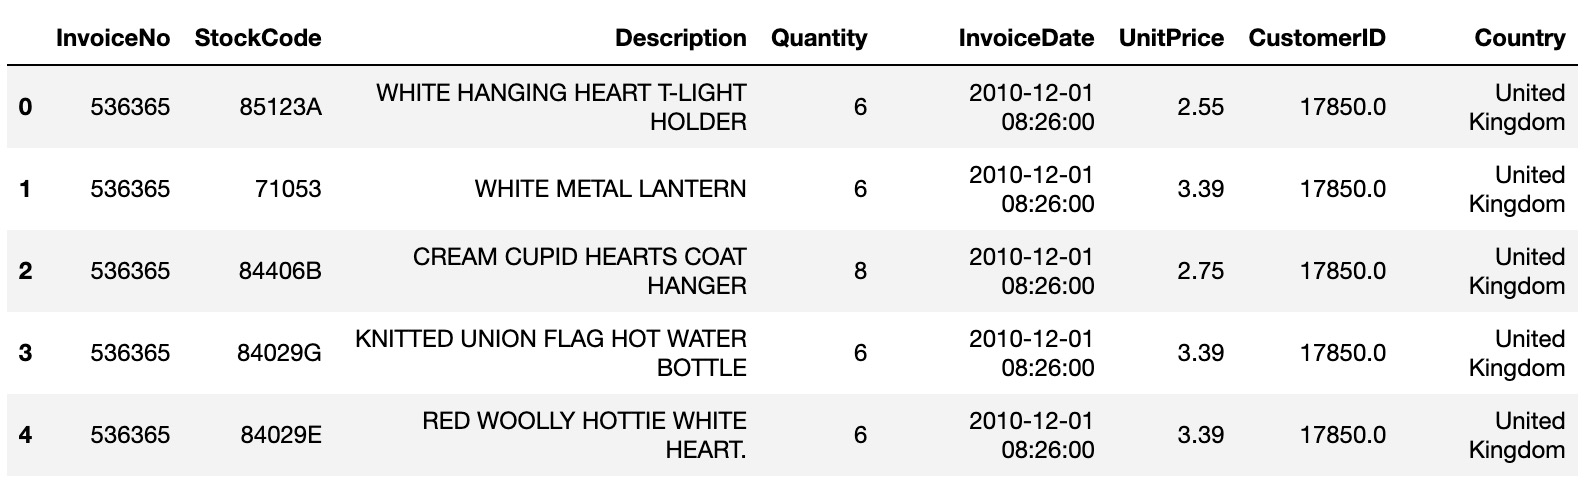
\includegraphics[width=\columnwidth]{sample}
 \caption{Sample Data from Online Retail Dataset}
 \end{figure}


\begin{table}[]
\centering
\caption{Online Retail Dataset Statistics}
\label{tab:my-table}
\resizebox{\columnwidth}{!}{%
\begin{tabular}{c|c|c|c|}
\cline{2-4}
                                     & \textbf{Quantity} & \textbf{UnitPrice} & \textbf{CustomerID} \\ \hline
\multicolumn{1}{|c|}{\textbf{count}} & 541,909           & 541,909            & 406,829             \\ \hline
\multicolumn{1}{|c|}{\textbf{mean}}  & 9.552250          & 4.611114           & 15287.69057         \\ \hline
\multicolumn{1}{|c|}{\textbf{std}}   & 218.081158        & 96.759853          & 1713.600303         \\ \hline
\multicolumn{1}{|c|}{\textbf{min}}   & -80995            & -11062.06          & 12346               \\ \hline
\multicolumn{1}{|c|}{\textbf{25\%}}  & 1                 & 1.25               & 13953               \\ \hline
\multicolumn{1}{|c|}{\textbf{50\%}}  & 3                 & 2.08               & 15152               \\ \hline
\multicolumn{1}{|c|}{\textbf{75\%}}  & 10                & 4.13               & 16791               \\ \hline
\multicolumn{1}{|c|}{\textbf{max}}   & 80995             & 38970              & 18287               \\ \hline
\end{tabular}%
}
\end{table}


\textbf{RFM Analysis:} The Recency, Frequency, and Monetary (RFM) research methodology is an extremely effective and well-known one for consumer segmentation. Customers are often divided based on their previous actions.

\textbf{Recency:} Recency alludes to the latest recent acquisition a client made. It refers to how often times a buyer awaits before making subsequent purchase. A lower value suggests that consumers make purchases or visits to the online store more frequently. Similar to this, a higher value denotes that a customer is much less likely to visit the business soon.

\textbf{Frequency:} Frequency is a measurement of how frequently a consumer made a purchase over a given time frame. Higher value suggests that clients are more devoted to the business, and lower value suggests the opposite.

\textbf{Monetary:} Money spent by a consumer during the specified time period is referred to as monetary. A higher value suggests that the company will receive more income and the lower value vice versa.

\textbf{Loyal Customers:} A set of customers just made a purchase, with a higher average for the number of transactions and amount spent.

\textbf{Lost Customers:} Group of clients with fewer transactions and less money spent overall than average who have not made a purchase.

\textbf{New Customers:} A group of clients who just made a purchase and whose number of transactions and overall spending is below normal.

\textbf{Prospect Customers:} A group of clients that recently made a purchase with a lot of transactions but below-average spending overall.

RFM scores are created by combining the recency, frequency, and monetary values. For instance, there are around 125 possible RFM possible scores in a five category rating system, with 555 being the maximum conceivable RFM score. RFM scores make the classifications of various clients very obvious. These RFM scores can be used by businesses to target specific clients with various marketing initiatives.

\textbf{Clustering Algorithms for Segmentation:} A method of unsupervised learning called clustering involves categorizing the raw data in order to find the underlying patterns in the data. Data points are divided into fewer clusters using clustering so that objects inside a cluster are very similar to one another and very discordant with objects in other clusters.

\textbf{K-Means Clustering Algorithms:} In the field of data mining, K-Means is a well-known unsupervised, iterative partitioning learning algorithm. It is used to solve several clustering issues, particularly for big datasets. The algorithm is divided into two sections. K centers are randomly chosen in the first section. K starts out fixed. Every data record is brought to the closest center in the second section. Self-organizing maps can be utilized to select the K’s starting value. By transforming high-dimensional data into a lower-dimensional space, the selforganizing map (SOM) data visualization technique aids in understanding high-dimensional data. By combining related items, it also illustrates the concept of clustering. The selforganizing map can be used to find the value of K that will be input into the k-means algorithm.

Euclidian distance metric is typically used to calculate the distance between two data points (the data item and the cluster center point). The following is the Euclidian function utilized by K-Means.

\begin{center}
E = $\sum_{i=1}^{k}$ $\sum_{x \in C_i}|x - x_i|^2$
\end{center}

\textbf{DBSCAN Algorithm: } Two epsilon (eps) and minimal point parameters are used by DBSCAN. The stages that this algorithm goes through are:

\begin{enumerate}
	\item As a candidate for the core point, choose any point or object at random from the data collection.
	\item The chosen item will create a new cluster with its neighboring object if it meets the criteria for a core point with the minimum and maximum values that the user has given. The euclidean distance formula is used to determine the separation between a corepoint object and a neighbor object as demonstrated below.
	\begin{center}
	$d_{xy} = \sqrt{ \sum_{i=1}^{n}(x_i - y_i)^2}$
	\end{center}
	
	\item The next corepoint candidate will be created for any objects that were not included as corepoints or surrounding  objects in stage 2. If it forms a corepoint, the object and its neighboring object will create the following cluster. Continuing until all of the data set’s objects have been tested.
\end{enumerate}

\textbf{Tools and Techniques:} This paper consists of the customer segmentation process. For this purpose different kinds of tools have been used. In the modern scenario, different advanced machine learning and deep learning-based tools have occupied the market for customer segmentation. Python is used for the visualization of this segmentation process. But in this project customer segmentation is done by a comparative study using K-Means and DBSCAN clustering techniques.  A very useful python library, “pandas”, is used for analyzing data and machine learning purposes. Numpy helps to handle multi-dimensional data. Seaborn is another library that helps to visualize graphs by providing some attractive themes. Matplotlib creates plotted graphs by analyzing the dataset. The Date Time module helps to manipulate dates and times to implement customer segmentation. For clustering purposes, different algorithms are used. In this project a web-based code editor, Jupyter Notebook is used which provides a very simplified visualized interface (Chindyana et al. 2021). 

\textbf{Data Collection:} Data collection is the most important part of differentiation from the customers. In this process, the transactional dataset used belongs to online retail companies. The data of customers is verified as all the details are taken from the ideal clients of the companies. It helps to understand the actual necessity of the customer and better understand them. In this data collection process, it is very important to take all the necessary information of the clients which includes invoice no, stock code, name, and details of customer’s purchased products, the quantity of the products, the actual date of making the invoice, customers country and the most important the customer id. 

\textbf{Data Analysis:} More than one hundred clustering algorithms are used for segmentation purposes. But few of them are popular till now. But the most widely used methods for making segments are K-means and Density-based spatial clustering of applications with noise (DBSCAN) Clustering. When the data is unsupervised and iterative we use the K-means data mining approach. The DBSCAN is a comparative data approach process. The k-means clustering process aims to cluster customers by observing the data. The main advantage of using the K-means data mining approach is that it can cluster a large amount of data very efficiently. The iterative algorithm of K-means can make clusters in different segments by analyzing the attributes of the customers. That categorized the data into different groups in a convenient way, unlike machine learning which needs training over time for accuracy. K-means has a centroid-based algorithm that makes each cluster by attaching a centroid. The main purpose for associating centroids is to minimize the total distances between each cluster and their corresponding dataset.

Though the same approaches are used for all clustering, the DBSCAN clustering method is used for creating arbitrarily shaped clusters. K-means fails to create this. DBSCAN clustering is capable of forming clusters that are based on varying densities. In this clustering method, the clusters are made in dense regions in space that are separated by lower-density regions. The most interesting feature of this clustering is that the number of clusters is not required beforehand unlike K-means. DBSCAN consists of two parameters “epsilon” and “minPoints”. “Epsilon” refers to the radius of the circle of each data point which is used to check density and “minPoints” refer to the lowest number of data points that are required inside the circle (Shirole et al. 2021).

\section{The results}
 
 To complete the data analysis first the library functions are imported into the Jupyter notebook. The following figure describes the imported functions such as the NumPy function; it is the library function of python that gives the ability to work with the arrays. The library function is beneficial for linear algebra, Fourier transforms, and matrix work (Marisa et al. 2019).

 \begin{figure}[h]
\centering
 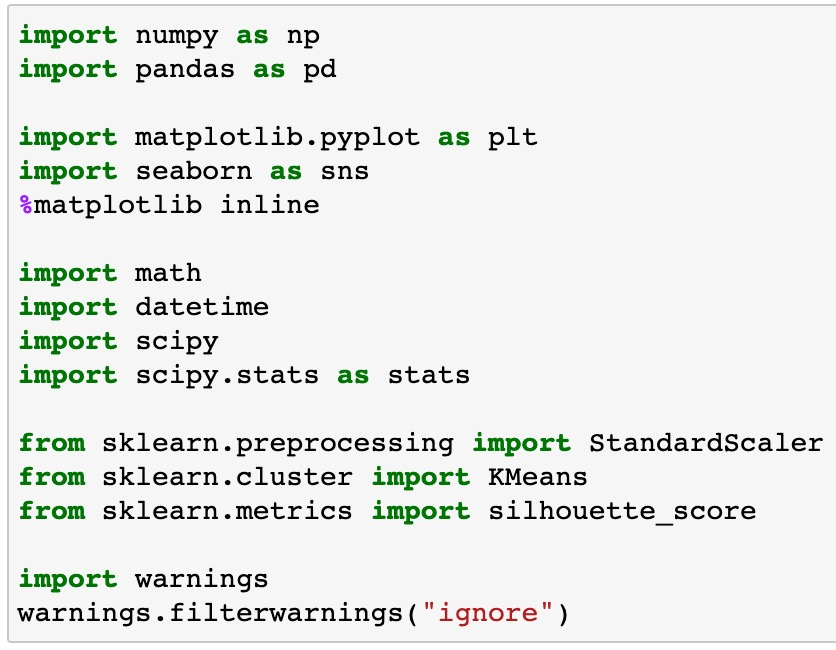
\includegraphics[width=6cm]{libs}
 \caption{Importing Library Functions}
 \end{figure}
 
 In 2005 Travis Oliphant created it and this is an open-source project; here numpy stands for numerical python. In this work, numpy is defined as np for making the work easier. Another important function is pandas which are defined in this work as ``pd'', this library function is important in analyzing the data (Koul et al. 2021). This library function is very useful for creating the data frame, importing CSV files, and preparing datasets. To visualize the data another important function that is used is matplotlib as this is an important function for such a purpose; this is defined in this work as “plt”.

 \begin{figure}[h]
\centering
 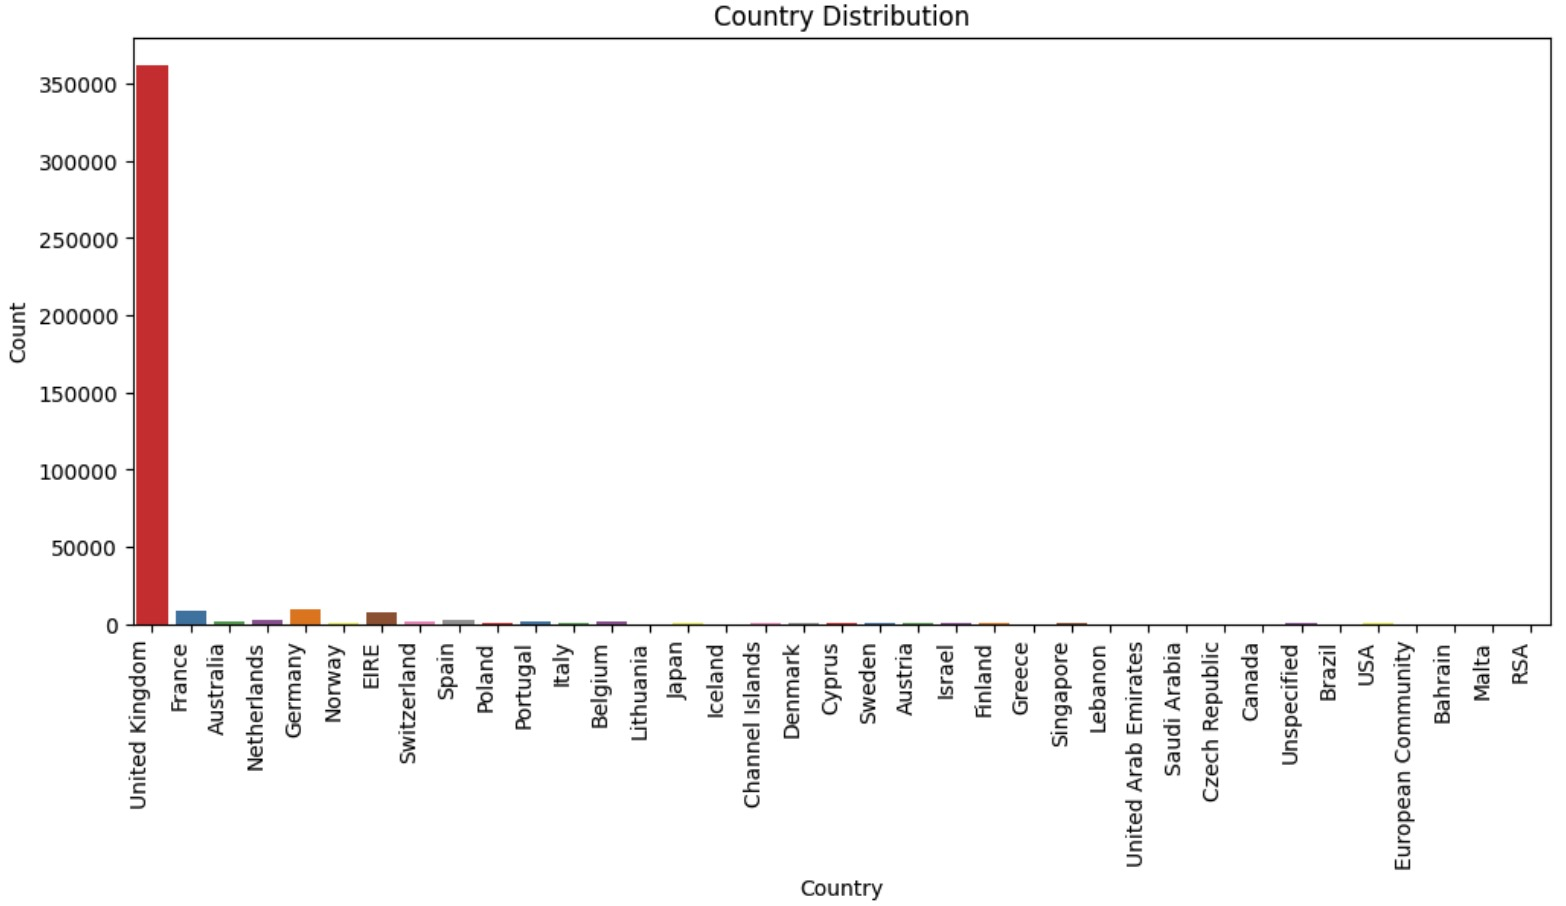
\includegraphics[width=9cm]{cntry_dist}
 \caption{Country Distribution Analysis}
 \end{figure}
 
  \begin{figure}[h]
\centering
 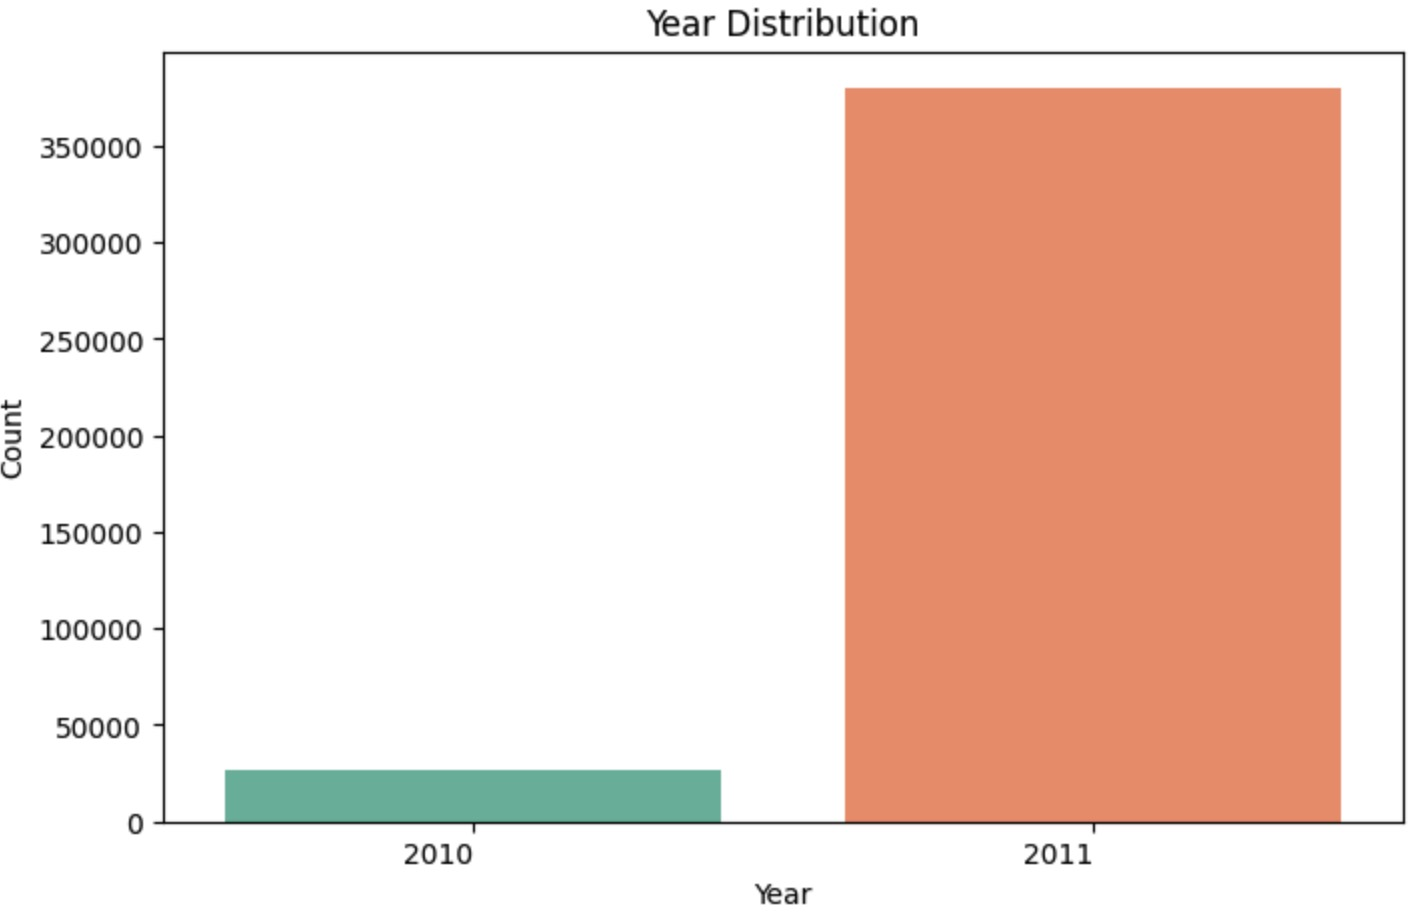
\includegraphics[width=9cm]{year_dist}
 \caption{Year Distribution Analysis}
 \end{figure}
 
  \begin{figure}[h]
\centering
 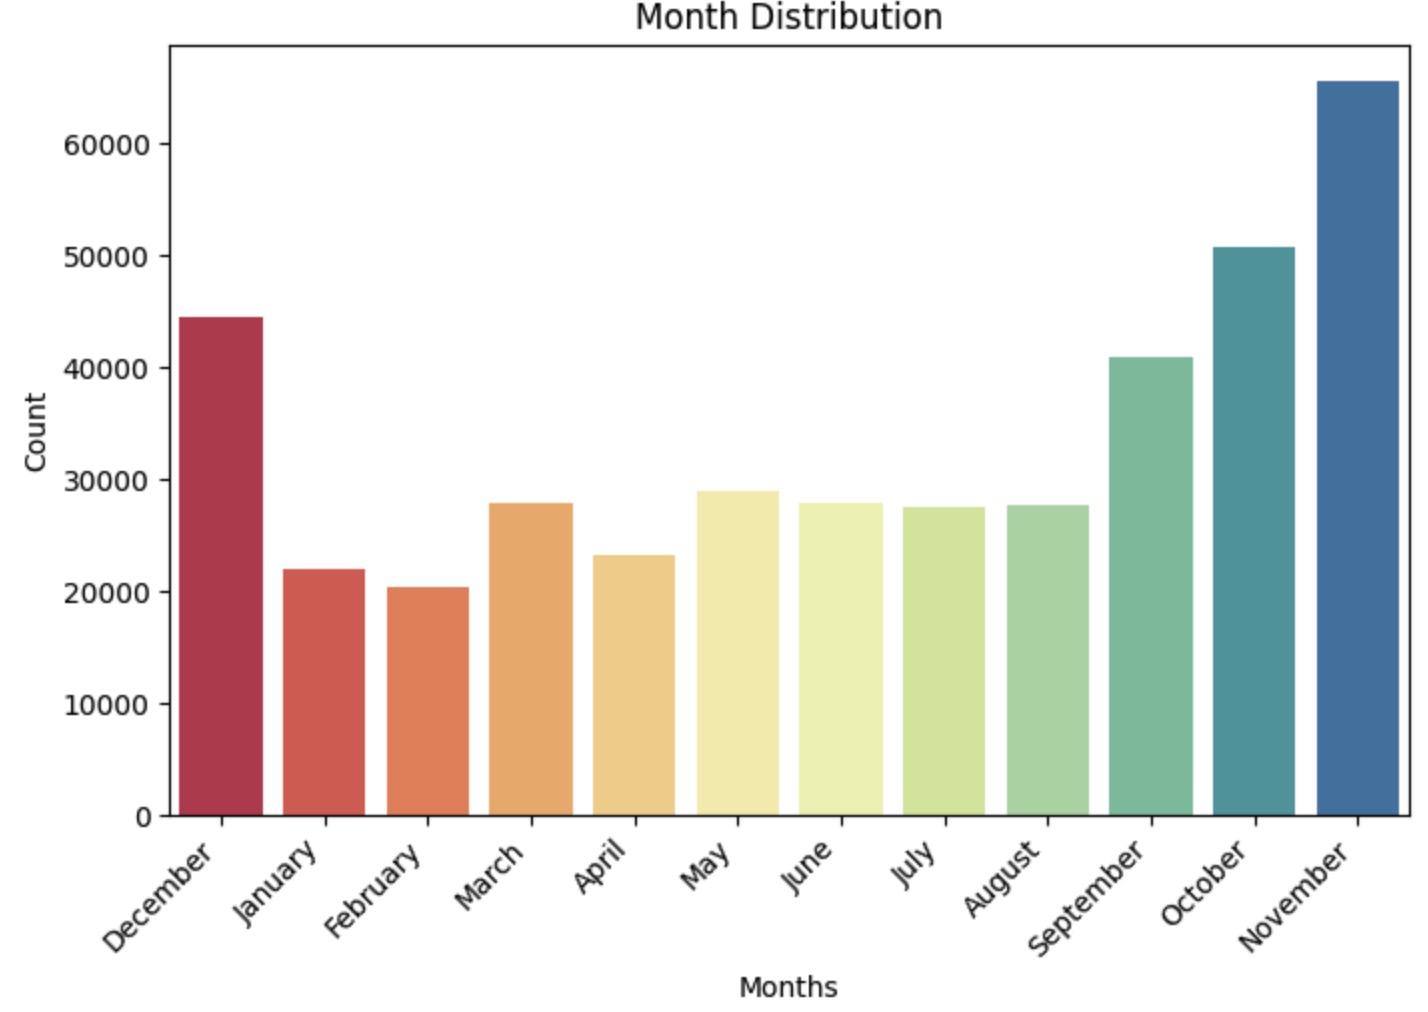
\includegraphics[width=9cm]{month_dist}
 \caption{Monthly Distribution Analysis}
 \end{figure}
 
   \begin{figure}[h]
\centering
 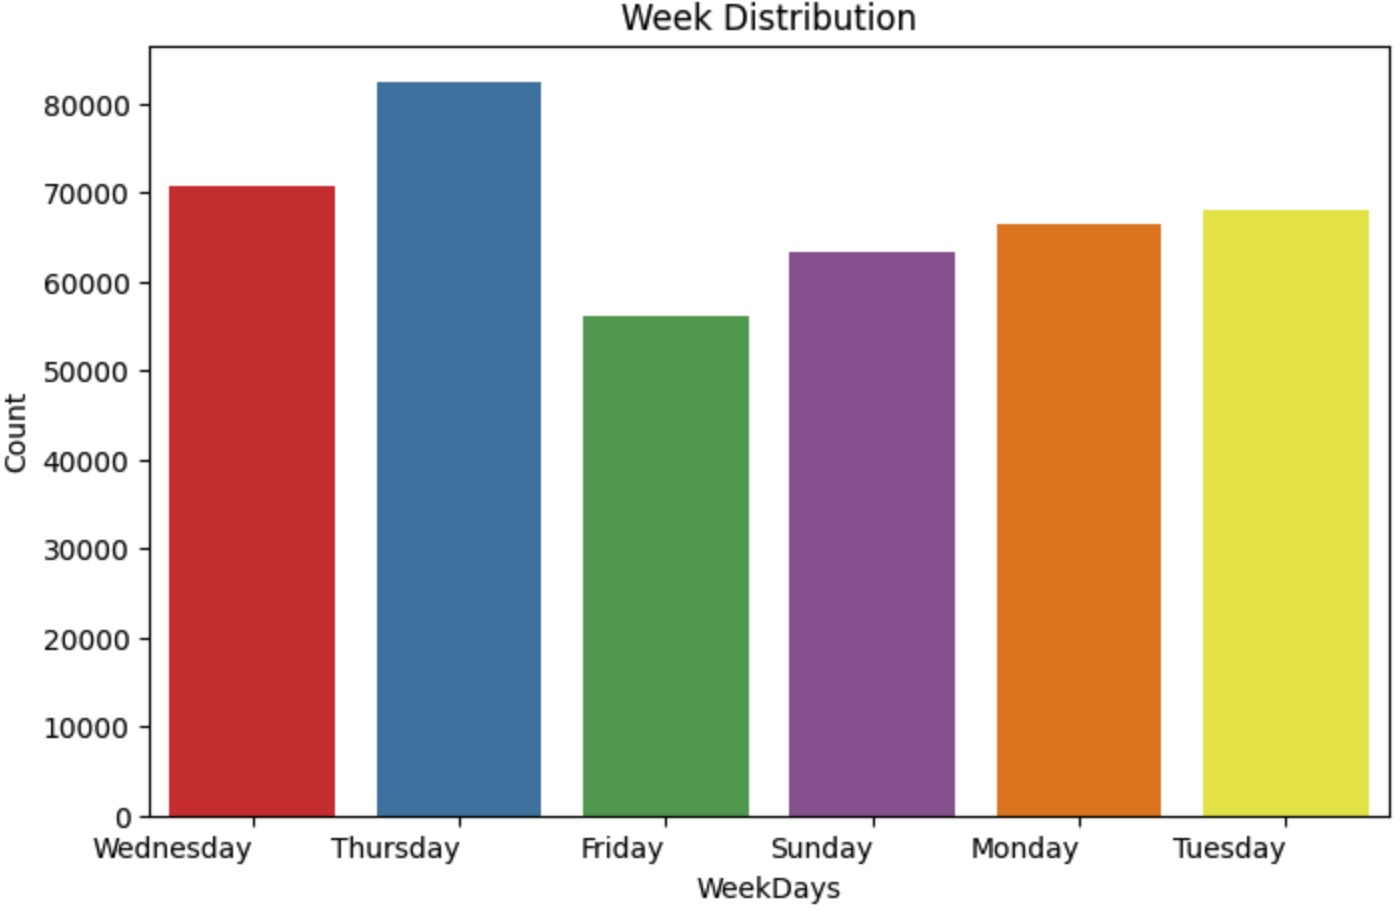
\includegraphics[width=9cm]{week_dist}
 \caption{Daywise Distribution Analysis}
 \end{figure}


 
 In this research work, the analysis on the online retail dataset is represented using several diagrams and all this analysis was completed in a Jupyter notebook. The analysis for the weekly, monthly, year-wise, and country-wise is done. The weekly analysis says that the weekly distribution is the highest on Thursday and it is represented by the blue colour. The second highest weekly distribution is Wednesday, which is represented by red colour. The monthly distribution says that the distribution is highest in November and it is represented by the deep blue colour. The second highest is October month which is represented by the specified colour. Here is the respective monthly distribution for the other months also represented. The yearly distribution analysis tells the analysis report is highest in 2011 and the graph is generated for only two years 2010 and 2011. The country distribution analysis report says that the United Kingdom has the highest data Amazon the respective countries.

Fig.7. Cluster vs SSD figures shows that the graph starts settling for the n-value ``2'. K-Means Algorithm is implemented for a range of values starting from 2 until 10. Silhouette scores for all the range of clusters were calculated to analyze each of the cluster. From both the SSD figure and the silhouette score analysis, cluster size n =2 is considered for K-Means Algorithm

 \begin{figure}[h]
\centering
 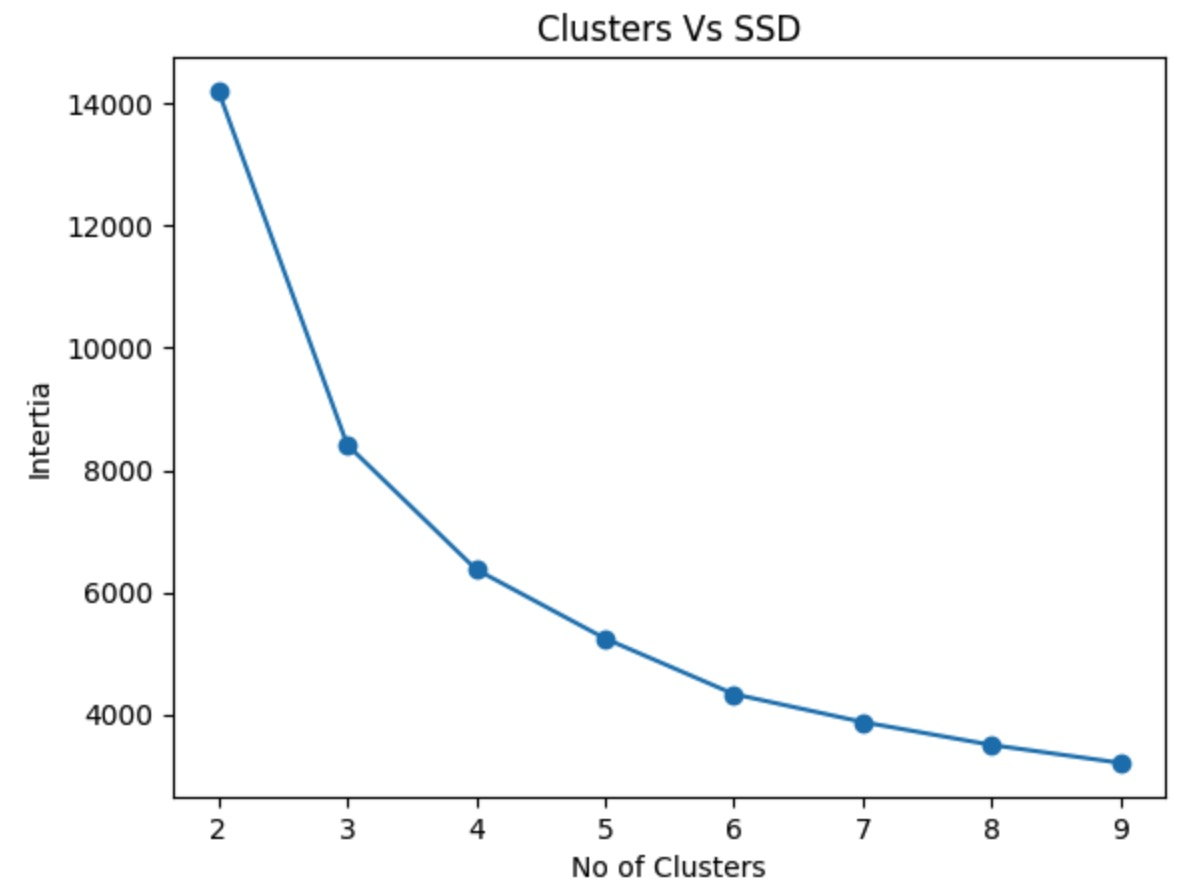
\includegraphics[width=9cm]{elbow}
 \caption{Cluster vs SSD}
 \end{figure}
 
  \begin{figure}[h]
\centering
 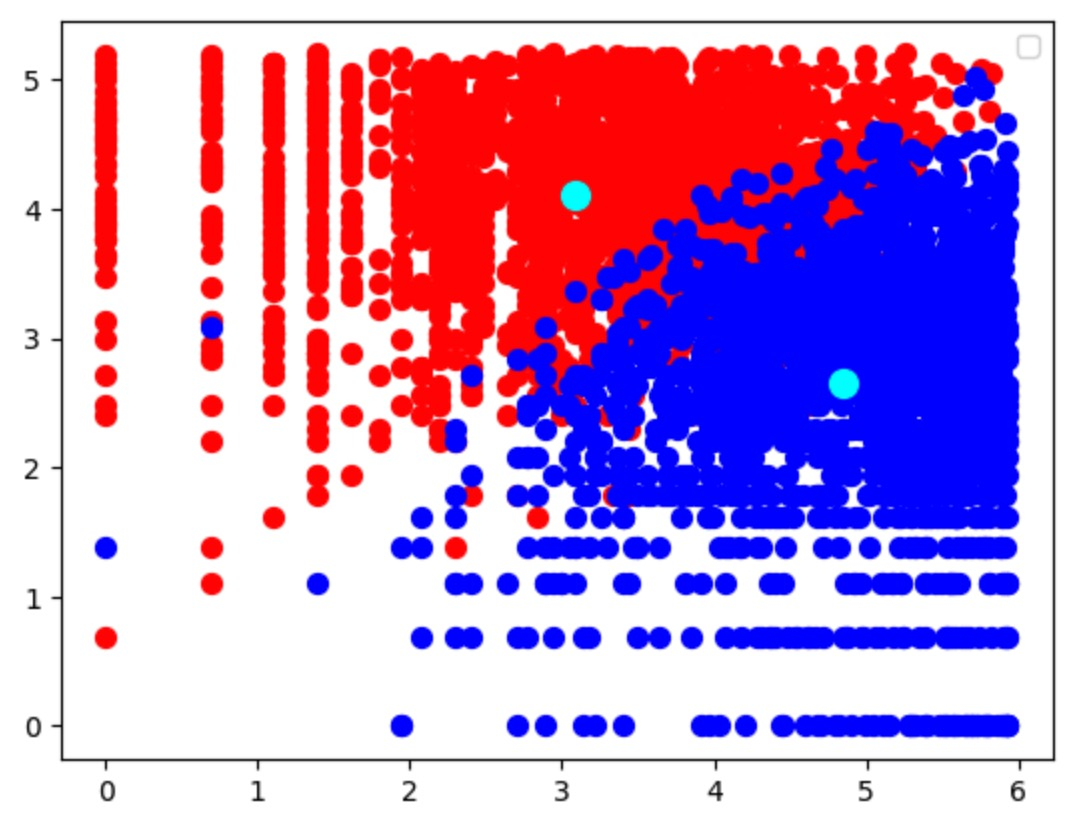
\includegraphics[width=9cm]{km}
 \caption{K-Means Clustering (2 Clusters with their centroids)}
 \end{figure}
 
 In Similar way, the same processed RFM dataset is used with DBSCAN Algorithm. DBSCAN predicted 4 different clusters/labels based on the data points available in the dataset with majority of the data points belonging to single cluster. Silhouette score for the DBSCAN algorithm is lesser than the K-Means clusters where as runtime for the DB scan is comparitively more than the K-Means for this dataset. Fig 8. represents the comparison between the two algorithms with their corresponding silhouette scores and average runtime for the algorithm to fit the model.
 
   \begin{figure}[h]
\centering
 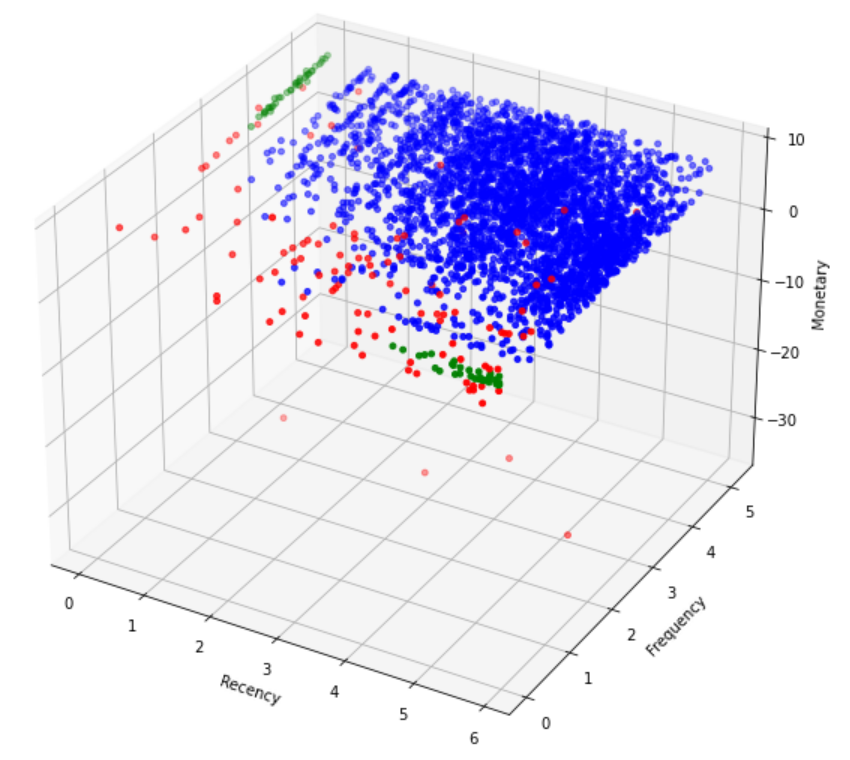
\includegraphics[width=9cm]{db}
 \caption{DBSCAN Clusters}
 \end{figure}
 
   \begin{figure}[h]
\centering
 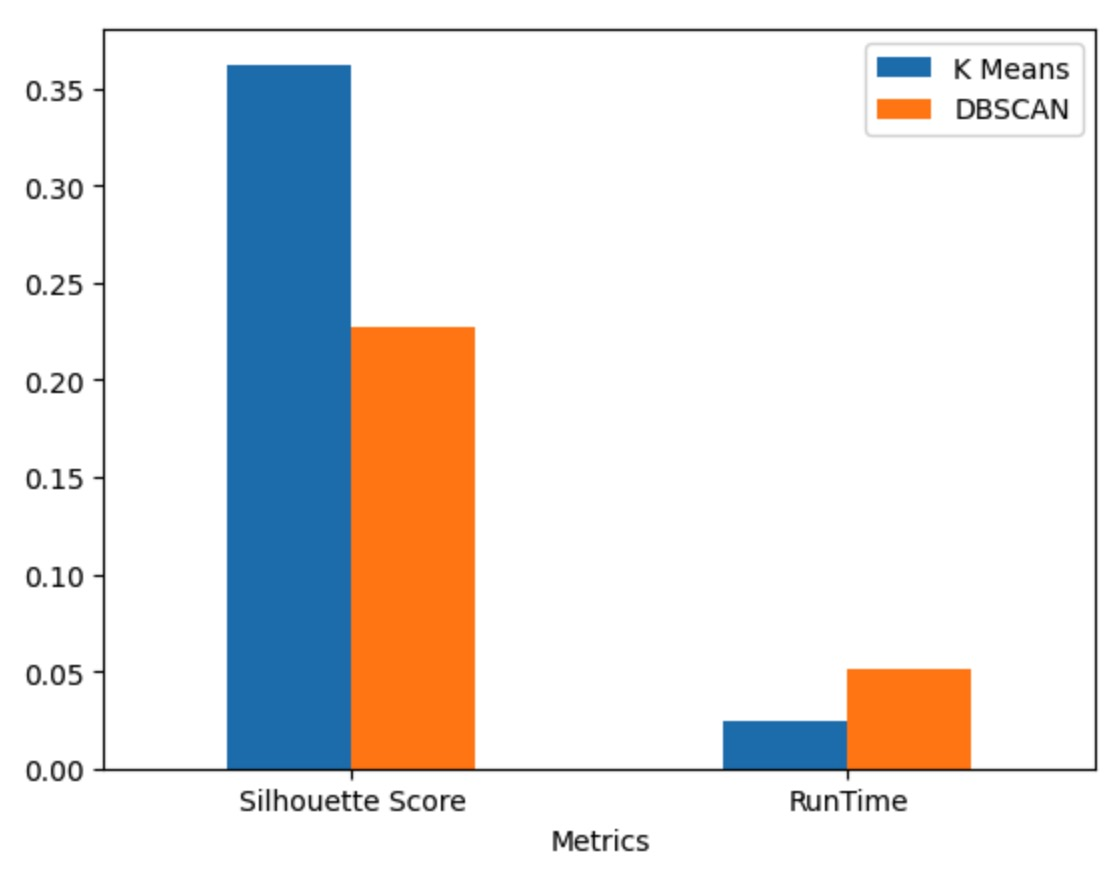
\includegraphics[width=9cm]{results}
 \caption{K-Means vs DBSCAN}
 \end{figure}
 

\section{Conclusion}

In this competitive market, companies are required to make new products based on customer's age, occupation, gender, taste, culture, geography, and preferences which will also help to retain the customer’s attention. In this case study, customer segmentation has been made so that companies can make products according to the customers' desires. K-means and DBSCAN clustering algorithms are used to differentiate the customer by analyzing the dataset that contains the information about clients. In this work, the segmentation of customers is calculated from the raw dataset. It will help the companies create more attractive advertisements, optimize the prices of the product, and improve the distribution channel. Different tools and techniques are used for this process. K-Means Algorithm performed better in both generating the clusters and also the time it takes to model the data for the online retail dataset compared to DBSCAN Clustering Algorithm.

\begin{thebibliography}{00}
	\bibitem{b1} Anthony O. Otiko, John A. Odey and Gabriel A. Inyang. ``Conceptualization of Market Segmentation and Patterns for Pre-Christmas Sales in an Online Retail Store.'' Journal of Science, Engineering and Technology, Vol. 6 (1), pages 51-59, 2019.
	\bibitem{b2} Mohamad Abdul Kadir and Adrian Achyar. ``Customer Segmentation on Online Retail using RFM Analysis: Big Data Case of Bukku.id.'' International Conference on Environmental Awareness for Sustainable Development in conjunction with International Conference on Challenge and Opportunities Sustainable Environmental Development. 2019.
	\bibitem{b3} A. Joy Christy, A. Umamakeswari, L.Priyatharsini and A. Neyaa. ``RFM ranking – An effective approach to customer segmentation.`` Journal of King Saud University – Computer and Information Sciences. 2018.
	\bibitem{b4} P. Anitha and Malini M. Patil. RFM model for Customer purchase behavior using K-Means Algorithm. Journal of King Saud University – Computer and Information Sciences. 2019.
	\bibitem{b5} Schellong Daniel , Kemper Jan and Brettel Malte. ``Clickstream Data as a source to uncover consumer shopping types in a large scale online setting.'' 2016.
	\bibitem{b6} Hadeel Ahmed, Bassam Kasasbeh, Balqees Aldabaybah and Enas Rawashdeh. ``Class balancing framework for credit card fraud detection based on clustering and similarity-based selection (SBS).'' 2022.
	\bibitem{b7} Wann Yih Wu, Phan Thi Phu Quyen and Adriana A. Amaya Rivas. ``How e-servicescapes affect customer online shopping intention: the moderating effects of gender and online purchasing experience.'' 2016
	\bibitem{b8} ASM Shahadat Hossain. ``Customer Segmentation using Centroid Based and Density Based Clustering Algorithms.'' International Conference on Electrical Information and Communication. 2017
	\bibitem{b9} Nassim Dehouche. ``Dataset on usage and engagement patterns for Facebook Live Sellers in Thailand.'' 2020.
	\bibitem{b10} Daqing Chen, Kun Guo and Bo Li. “Predicting Customer Profitability Dynamically over Time: An Experimental Comparative Study”. 2019..
	\bibitem{b11} Vinaya Manchaiah, Amyn M. Amlani, Christina M.Bricker, Clayton T. Whitfield and Pierre Ratinaud. “Benefits and Shortcomings of Directto-Consumer Hearing Devices: Analysis of Large Secondary Data Generated from Amazon Customer Reviews.” Journal of Speech, Language, and Hearing Research. 2019.
	\bibitem{b12} Gaurav Mishra and Sraban Kumar Mohanty. ``A fast hybrid clustering technique based on local nearest neighbor using minimum spanning tree.'' 2019.
	\bibitem{b13} Kayalvily Tabianan, Shubashini Velu and Vinayakumar Ravi. “K-Means Clustering Approach for Intelligent Customer Segmentation Using Customer Purchase Behavior Data”. 2022.
	\bibitem{b14} Danuta Zakrzewska and Jan Murlewski. “Clustering Algorithms for Bank Customer Segmentation”. 2005
	\bibitem{b15}  Jun Wu, Wen-Pin Lin, Sang-Bing Tsai, Yuanyuan Li, Liping Yang and Guangshu Xu. “An Empirical Study on Customer Segmentation by Purchase Behaviors  sing a RFM Model and K-Means Algorithm.” 2020.
	
\end{thebibliography}



\end{document}